\documentclass[tikz,border=10pt]{standalone}

% Essential packages for TikZ
\usepackage{tikz}
\usepackage{graphicx}
\usepackage{amsmath}
\usepackage{calc}

% Additional TikZ libraries that might be needed
\usetikzlibrary{positioning,calc,arrows.meta}

% Define the \scalebox command if not using the graphicx package already
\usepackage{graphics}

% Document begins
\begin{document}

\begin{tikzpicture}
% Styles
%\tikzstyle{label}=[font=\tiny]
\tikzstyle{arr}=[->,-latex,line width=1pt]
% The left image (reactants) - moved further left
\node[anchor=center,inner sep=0] (image) at (-20,0){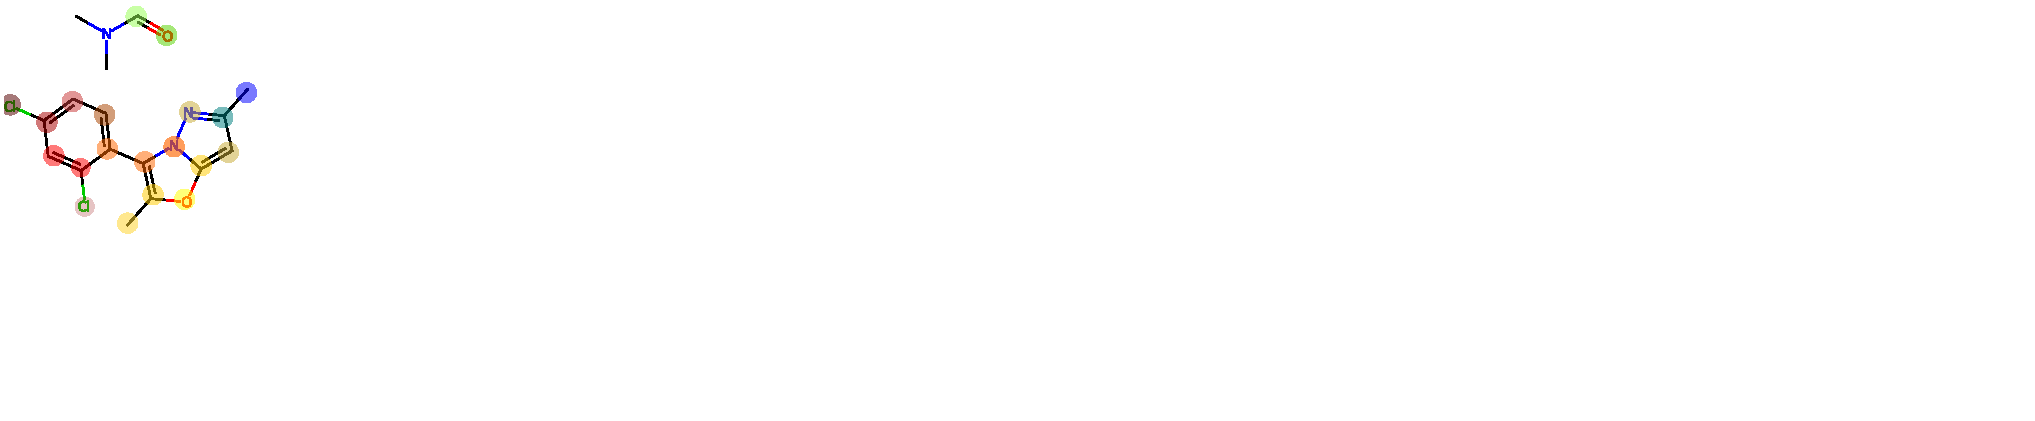
\includegraphics[width=10cm,height=6cm,keepaspectratio]{fig/reactants.pdf}};
\node[anchor=center,inner sep=0](drawing) at (0.2,0){
\includegraphics[width=1cm,height=2cm,keepaspectratio]{fig/dots.pdf}};
\node[anchor=center,inner sep=0] (drawing) at (-2.6,0){
\includegraphics[width=3cm,height=5cm,keepaspectratio]{fig/arrows.pdf}};
\node[anchor=center,inner sep=0] (drawing) at (-8,0){
\includegraphics[width=10cm,height=7cm,keepaspectratio]{fig/noisy.pdf}};
\node[anchor=center,inner sep=0] (drawing) at (-13.5,0){
\includegraphics[width=3cm,height=5cm,keepaspectratio]{fig/arrows.pdf}};
\node[anchor=center,inner sep=0] (drawing) at (-16,0){
\includegraphics[width=1cm,height=2cm,keepaspectratio]{fig/dots.pdf}};
% The right image (product) - moved further right
\node[anchor=center,inner sep=0] (drawing) at (6,0){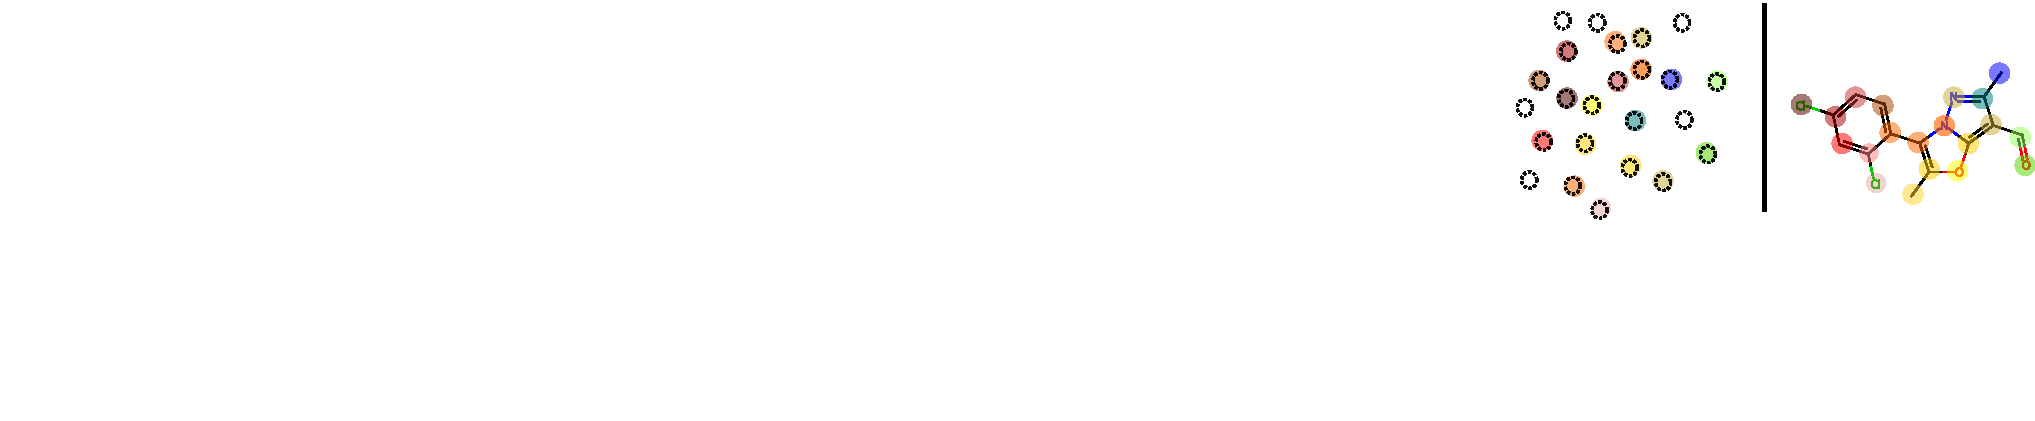
\includegraphics[width=10cm,height=7cm,keepaspectratio]{fig/product.pdf}};
% Scope for drawing on image
% Labels
\node[text width=10cm, align=center] at (-20,4) {Target (reactants)};
\node[text width=10cm, align=center] at (8,4) {Input (product)};
\node[text width=1cm, align=center] at (8.5,-4) {$\Y$};
\node[text width=1cm, align=center] at (3.5,-4) {$\X_T$};
\node[text width=1cm, align=center] at (-8,-4) {$\X_t$};
\node[text width=1cm, align=center] at (-20,-4) {$\X_0$};
\node (c0) at (-2.6,0) {};
\node[text width=1cm, align=center] at ($(c0) + (-1,2)$) {\scalebox{.7}{$q(\X_t\!\mid\!\X_{t-1})$}};
\node[text width=1cm, align=center] at ($(c0) + (-1,-2)$) {\scalebox{.7}{$p_\theta(\X_{t-1}\!\mid\!\X_t,\!\Y)$}};
\node[text width=1cm, align=center] at ($(c0) + (1,-6)$) {\scalebox{.7}{$=\sum_{\X_0}q(\X_0\!\mid\!\X_T,\!\X_0)p_\theta(\X_{0}\!\mid\!\X_{T},\!\Y,\!\P^{\Y\to\X})$}};
\node (c0) at (-13.5,0) {};
\node[text width=1cm, align=center][text width=1cm, align=center][text width=1cm, align=center] at ($(c0) + (-2,2)$) {\scalebox{.7}{$q(\X_{t+1}\!\mid\!\X_{t})$}};
\node[text width=1cm, align=center] at ($(c0) + (-2,.-2)$) {\scalebox{.7}{$p_\theta(\X_{t}\!\mid\!\X_{t+1},\!\Y)$}};
\end{tikzpicture}

\end{document}